\documentclass[border=0mm]{standalone}

\usepackage{contour}
\usepackage{ifthen}
\usepackage{tcolorbox}
\usepackage{tikz}
\usepackage{xcolor}

%%%%%%%%%%%%%%%%%%%%%%%%%%%%%%%%%%%%%%%%%%%%%%%%%%%%%%%%%%%%%%%%%%%%%%%%%%%%%
% File: colours.tex
% Author: Edmund Mulligan <edmund@edmundmulligan.name>
% Version: 1.0
% This file is part of the workbook for Non-Violent Communication.
% Description: Contains the definitions of the colours used in the workbook.
%%%%%%%%%%%%%%%%%%%%%%%%%%%%%%%%%%%%%%%%%%%%%%%%%%%%%%%%%%%%%%%%%%%%%%%%%%%%%
\definecolor{tem_cyan}{rgb}{.2, .8, .8}
\definecolor{tem_purple}{rgb}{0.706, 0.051, 0.831}
\definecolor{tem_grey}{RGB}{245, 245, 245}

 \definecolor{tem_blue1}{RGB}{240,248,255} % AliceBlue
 \definecolor{tem_blue2}{RGB}{135,206,250} % LightSkyBlue
 \definecolor{tem_blue3}{RGB}{100,149,237} % CornflowerBlue
 \definecolor{tem_blue4}{RGB}{0,0,255}     % Blue
 \definecolor{tem_blue5}{RGB}{0,0,128}     % Navy


\begin{document}
  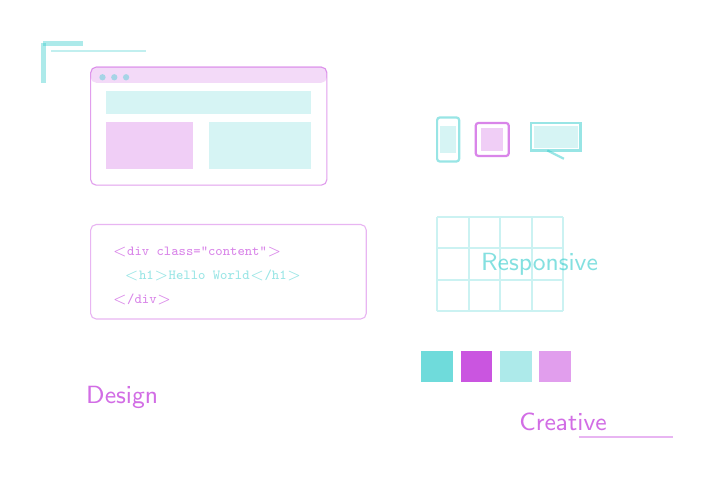
\begin{tikzpicture}
    % Business card dimensions: 85mm x 55mm (approx 8.5cm x 5.5cm)
    % Define the card background
    \fill[white] (0,0) rectangle (8.5,5.5);
    
    % Browser window mockup (top)
    \begin{scope}[shift={(0.8,3.5)}]
      % Browser chrome
      \draw[tem_purple, opacity=0.4, rounded corners=2pt] (0,0) rectangle (3.0,1.5);
      \fill[tem_purple, opacity=0.15, rounded corners=2pt] (0,1.3) rectangle (3.0,1.5);
      % Browser dots
      \fill[tem_cyan, opacity=0.4] (0.15,1.37) circle (0.04);
      \fill[tem_cyan, opacity=0.4] (0.30,1.37) circle (0.04);
      \fill[tem_cyan, opacity=0.4] (0.45,1.37) circle (0.04);
      % Content area with simple layout
      \fill[tem_cyan, opacity=0.2] (0.2,0.9) rectangle (2.8,1.2);
      \fill[tem_purple, opacity=0.2] (0.2,0.2) rectangle (1.3,0.8);
      \fill[tem_cyan, opacity=0.2] (1.5,0.2) rectangle (2.8,0.8);
    \end{scope}
    
    % Responsive design icons (mobile, tablet, desktop)
    \begin{scope}[shift={(5.2,3.8)}, scale=0.7]
      % Mobile
      \draw[tem_cyan, thick, opacity=0.5, rounded corners=1pt] (0,0) rectangle (0.4,0.8);
      \fill[tem_cyan, opacity=0.2] (0.05,0.15) rectangle (0.35,0.65);
      % Tablet
      \draw[tem_purple, thick, opacity=0.5, rounded corners=1pt] (0.7,0.1) rectangle (1.3,0.7);
      \fill[tem_purple, opacity=0.2] (0.8,0.2) rectangle (1.2,0.6);
      % Desktop
      \draw[tem_cyan, thick, opacity=0.5] (1.7,0.2) rectangle (2.6,0.7);
      \draw[tem_cyan, thick, opacity=0.5] (2.0,0.2) -- (2.3,0.05) -- (2.3,0.05);
      \fill[tem_cyan, opacity=0.2] (1.75,0.25) rectangle (2.55,0.65);
    \end{scope}
    
    % Code snippet element
    \begin{scope}[shift={(0.8,1.8)}]
      \draw[tem_purple, opacity=0.3, rounded corners=2pt] (0,0) rectangle (3.5,1.2);
      \node[tem_purple, font=\tiny\ttfamily, opacity=0.5, align=left, anchor=west] at (0.15,0.85) 
        {\textless div class="content"\textgreater};
      \node[tem_cyan, font=\tiny\ttfamily, opacity=0.5, align=left, anchor=west] at (0.3,0.55) 
        {\textless h1\textgreater Hello World\textless/h1\textgreater};
      \node[tem_purple, font=\tiny\ttfamily, opacity=0.5, align=left, anchor=west] at (0.15,0.25) 
        {\textless/div\textgreater};
    \end{scope}
    
    % Color palette squares
    \begin{scope}[shift={(5.0,1.0)}]
      \fill[tem_cyan, opacity=0.7] (0,0) rectangle (0.4,0.4);
      \fill[tem_purple, opacity=0.7] (0.5,0) rectangle (0.9,0.4);
      \fill[tem_cyan, opacity=0.4] (1.0,0) rectangle (1.4,0.4);
      \fill[tem_purple, opacity=0.4] (1.5,0) rectangle (1.9,0.4);
    \end{scope}
    
    % Grid layout representation
    \begin{scope}[shift={(5.2,1.9)}, opacity=0.25]
      \draw[tem_cyan, thick] (0,0) grid[step=0.4] (1.6,1.2);
    \end{scope}
    
    % Friendly labels
    \node[tem_purple, font=\small\sffamily, opacity=0.6] at (1.2, 0.8) {Design};
    \node[tem_cyan, font=\small\sffamily, opacity=0.6] at (6.5, 2.5) {Responsive};
    \node[tem_purple, font=\small\sffamily, opacity=0.6] at (6.8, 0.5) {Creative};
    
    % Subtle decorative elements
    \draw[tem_cyan, thick, opacity=0.3] (0.3,5.2) -- (1.5,5.2);
    \draw[tem_purple, thick, opacity=0.3] (7.0,0.3) -- (8.2,0.3);
    
    % Small corner accent
    \draw[tem_cyan, line width=2pt, opacity=0.4] (0.2,5.3) -- (0.2,4.8);
    \draw[tem_cyan, line width=2pt, opacity=0.4] (0.2,5.3) -- (0.7,5.3);
    
  \end{tikzpicture}
\end{document}
